\subsection{Theory}
\begin{frame}[fragile]{\textbf{4. Krylov subspace}}

In general, a projection method for solving the linear system:
\[
\mathcal{A}x = b
\]

extracts an approximate solution $x^{(m)}$ from an affine subspace $x^{(0)}+\mathcal{K}^{(m)}$ of dimension $m$ by imposing the Petrov-Galerkin condition:
\[
b - \mathcal{A}x^{(m)} \bot \mathcal{L}^{(m)}
\]


where $\mathcal{L}^{(m)}$ is another subspace of dimension $m$.


Krylov methods are methods for which $\mathcal{K}^m$ is:
\[
\mathcal{K}^{(m)} (\mathcal{A},r^{(0)}) = \mathrm{span} \left\{ r^{(0)}, \mathcal{A}r^{(0)}, \mathcal{A}^2r^{(0)}, \mathcal{A}^{3}r^{(0)}, ... , \mathcal{A}^{m-1}r^{(0)}\right\}
\]

This is tricky and I won't be able to present this in much detail, but we will present two such methods:
\begin{itemize}
	\item Conjugate Gradient
	\item GMRES
\end{itemize}
\end{frame}

\subsection{Conjugate gradient }


\begin{frame}[fragile]{\textbf{4. CG algorithm}}
The conjugate gradient method is the simplest Krylov method (in my opinion). It is very efficient, but it only works for symmetric matrices. In the following, the scalar product is noted $(u,v)$.

\vspace{0.5cm}


  \begin{algorithm}[H]
	\KwIn{\begin{itemize}
			\item Given a starting point residual $r^{(0)}:=b-\mathcal{A}x^{(0)}$  and $p^{(0)}= r^{(0)}$
			\item Given a tolerance $\mathrm{tol}$ 
	\end{itemize}}

	Initialize $j=0$
	
	\While{ $\lVert r^{(j)} \rVert < \mathrm{tol}$}
	{
		$\alpha^{(j)} := \frac{(r^{(j)},r^{(j)})}{(\mathcal{A}p^{(j)},p^{(j)})} $
		
		$x^{(j+1)} := x^{(j)} + \alpha^{(j)}p^{(j)}$
		
		$r^{(j+1)} = r^{(j)} - \alpha^{(j)} \mathcal{A}p^{(j)}$
		
		$\beta^{(j)} = \frac{(r^{(j+1)},r^{(j+1)})}{(r^{(j)},r^{(j)})}$
		
		$p^{(j+1)} = r^{(j+1)} + \beta^{(j)} p^{(j)}$
		
	}
\end{algorithm}
\end{frame}


\begin{frame}
	\frametitle{\textbf{4. CG results}}
\centering
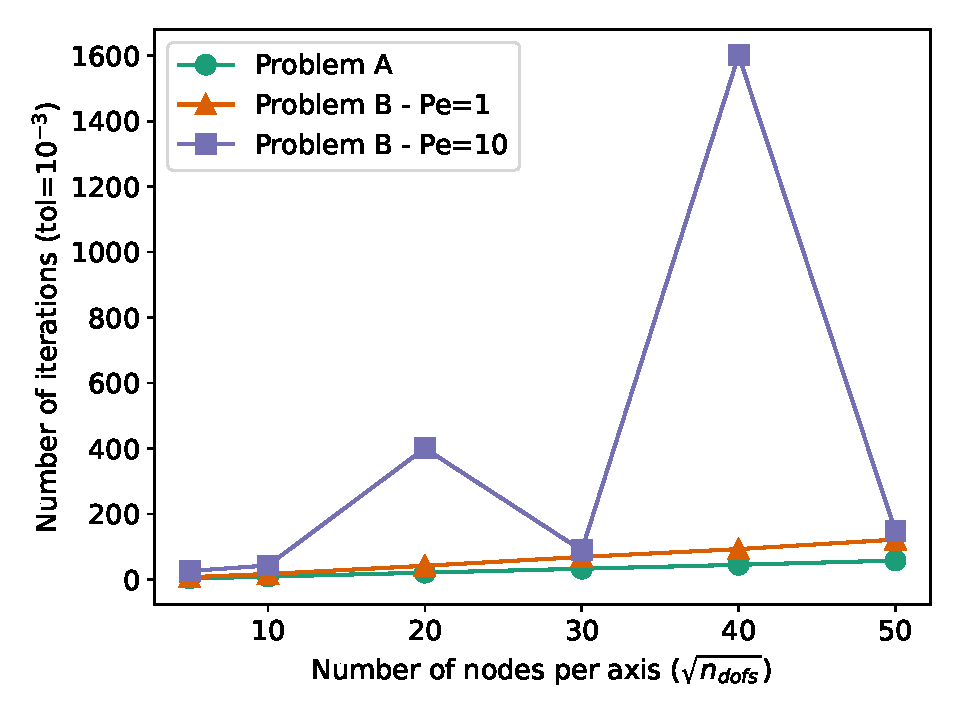
\includegraphics[width=0.95\linewidth]{images/cg_its}
\end{frame}

\subsection{GMRES}

\begin{frame}[fragile]{\textbf{4. GMRES}}
	The Generalized Minimal RESidual method (GMRES) is a projection method that aims a minimizing the residual norm over all the vectors of the Krylov subspace that is being built ($x^{(0)}+\mathcal{K}^{(m)}$).
	
	
	The GMRES algorithm uses the Arnoldi iteration for numerical stability. The Arnoldi iteration
%	produces Hn, an (n + 1) × n upper Hessenberg matrix, and Qn, a matrix whose columns make up an
%	orthonormal basis of Kn(A, b), such that AQn = Qn+1Hn. The GMRES algorithm nds the vector
%	xn which minimizes the norm kb − Axnk2
%	, where xn = Qnyn + x0 for some yn ∈ R
%	n. Since the
%	columns of Qn are orthonormal, the residual can be equivalently computed as
%	
%	 The algorithm is quite complex. I  give it here, but you will need to take a dive into the code to acquire a better understanding of it.
%	
	\vspace{0.5cm}
	
\end{frame}

\begin{frame}[fragile]{\textbf{4. GMRES Algorithm}}

\begin{algorithm}[H]
	\KwIn{A matrix $\mathcal{A}$, a RHS $b$, an initial guess $x^{(0)}$, a maximum number of Krylov vectors $p$ and a tolerance $\mathrm{tol}$}

	$\mathcal{Q}\leftarrow$empty(size($b$),$p+1$)
	
	$\mathcal{H}\leftarrow$empty($p+1$,$p$)
	
	$e_1 \leftarrow$ empty(size($b$),$p+1$) $ + [1,\dots,0]^T$
	
	$r^{(0)} = b-\mathcal{A}x^{(0)}$
	
	$\beta = \lVert r^{(0)} \rVert$

	
	$\mathcal{Q}_{:,0} = \frac{r^{(0)}}{\lVert r^{(0)} \rVert}$
	
	

	\For{$j=0 \dots p-1$}
	{
	   $\mathcal{Q}_{:,j+1} \leftarrow (\mathcal{A},\mathcal{Q}_{:,j})$
	   
	   \For{$i=0 \dots j$}{
	   	  $\mathcal{H}_{i,j} = (\mathcal{Q}^{T}_{:,i},\mathcal{Q}_{:,j+1})$
	   	   
	   	   $\mathcal{Q}_{:,j+1} \leftarrow  \mathcal{Q}_{:,j+1} - (\mathcal{A},\mathcal{Q}_{:,j})$
	   }
	   
	   $\mathcal{H}_{j+1,j} = \lVert \mathcal{Q}^{(j)} \rVert$
	   

	  
	  $\mathcal{H}_{:j+2,:j+1}^{T} \mathcal{H}_{:j+2,:j+1} y = \beta \mathcal{H}_{:j+2,:j+1}^{T}  e_1$
	
	  $x^{j+1} = x^{(0)} + \mathcal{Q}_{:,:j+1}$ y
	  
	  \If {$\lVert r^{(j+1)} \rVert < \mathrm{tol}$}
	  {
	  	\textbf{break}
	  }
	}
\end{algorithm}

\end{frame}

\begin{frame}
	\frametitle{\textbf{4. GMRES results}}
	\centering
	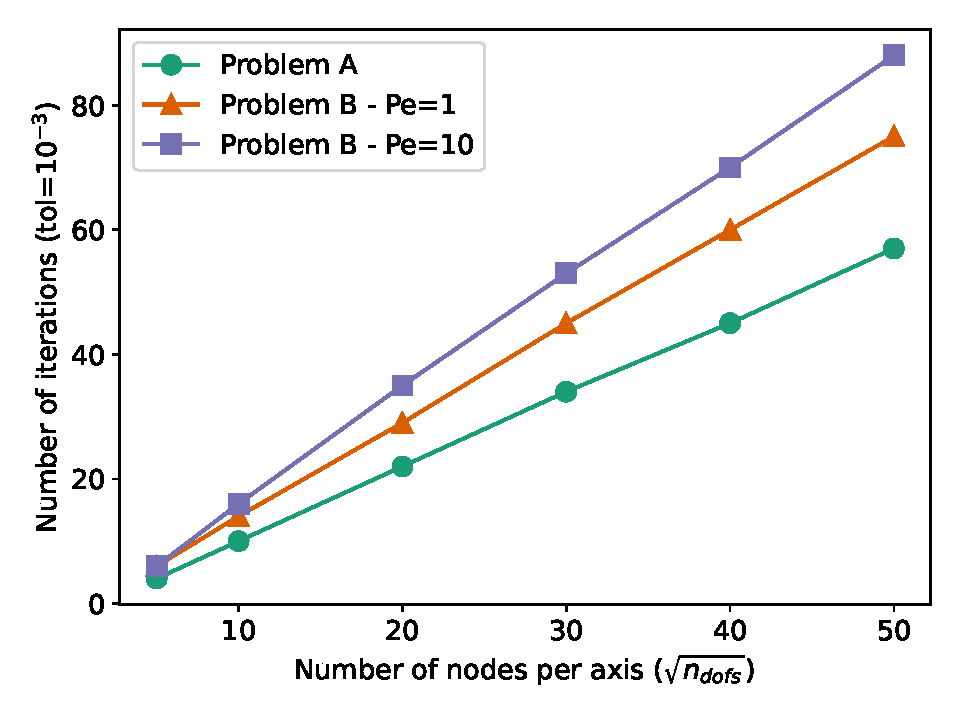
\includegraphics[width=0.95\linewidth]{images/gmres_its}
\end{frame}


